\chapter{Análisis y especificación}

El análisis es la fase de la ingeniería del software en la que se describen las características necesarias para llevar a cabo los objetivos planteados en el software que se va a desarrollar. Previa a la fase del diseño sirve para descubrir los conflictos existentes entre requisitos y conocer más a fondo el sistema a desarrollar.
\bigskip

Para el desarrollo de todos los diagramas que aparecen en esta sección se ha utilizado ArgoUML, una aplicación de software libre que se puede encontrar en \cite{ARG}.
\bigskip

\section{Actores}
Son los entes que interactúan con el sistema, pueden ser personas, programas u otros sistemas remotos. En el caso que nos ocupa sólo hay un tipo de actor que sería el usuario:
\bigskip

\begin{itemize}
\item \textbf{Usuario:}Será la persona que utilice el software final para llevar acabo análisis de grandes conjuntos de datos. Está encuadrado en un público objetivo como pueden ser investigadores que necesiten encontrar patrones en grandes conjuntos de datos, administradores de redes que quieran detectar ataques en sus sistemas, etc. 
La materia que se estudie es irrelevante mientras los datos se estructuren como el software los acepta.
\end{itemize}
\bigskip

\subsection{Ficha de descripción de actor}

\begin{table}[H]
\begin{center}
\resizebox{10cm}{!} {
\begin{tabular}{|c|c|c|}
\hline
Actor & Usuario & Usr	\\ \hline
Descripción &\multicolumn{2}{|c|}{Actor encargado de utilizar el sistema}	\\ \hline
Características & \multicolumn{2}{|c|}{No existen características previas necesarias}	\\ \hline
Relaciones & \multicolumn{2}{|c|}{No posee relaciones con otros actores}	\\ \hline
Referencias &\multicolumn{2}{|c|}{CU-1,CU-2,CU-3,CU-4,CU-5,CU-6,CU-7}	\\ \hline
\end{tabular}
}
\caption{Ficha de descripción de usuarios.}
\end{center}
\end{table}

\bigskip

Cada uno de los elementos que aparecen en la sección "Referencias" son los casos de uso que se explicaran a lo largo del presente capítulo.

\section{Requisitos}
\bigskip

\subsection{Requisitos no funcionales}

Son restricciones que afectan a las funciones del software, acotando el diseño. No definen las funciones si no las propiedades.

\begin{itemize}
\item \textbf{RNF-1:}El sistema debe estar desarrollado en MATLAB.
\item \textbf{RNF-2:}El sistema debe hacer uso de “MEDA-Toolbox”.
\item \textbf{RNF-3:}El sistema debe ser portable y multiplataforma.
\item \textbf{RNF-4:}Los datos de entrada deben ser validados.
\item \textbf{RNF-5:}Los errores en la introducción de datos deben ser capturados y notificados.
\item \textbf{RNF-6:}Todo el software desarrollado debe ser libre y accesible a la comunidad.
\end{itemize}

\bigskip

\subsection{Requisitos funcionales}
Los requisitos funcionales son las características que debe poseer el sistema para llevar a cabo todos los objetivos planteados y cubrir las necesidades de los usuarios que lo utilicen.

\begin{itemize}
\item \textbf{RF-1:}Procesamiento de los datos a analizar.
\item \textbf{RF-2:}Generación de modelos completos con toda la información.
\item \textbf{RF-3:}Generación de modelos intermedios para cada fichero de datos.
\item \textbf{RF-4:}Almacenamiento de la información del entorno en ficheros.
\item \textbf{RF-5:}Generación de Score Plots, MEDA y oMEDA.
\item \textbf{RF-6:}Carga de entornos desde ficheros.
\end{itemize}

\bigskip

\subsection{Requisitos de información}

Los requisitos de información están relacionados con los datos que el sistema necesita almacenar para su funcionamiento. En el caso que nos ocupa el sistema no necesita almacenar datos para funcionar, aunque brinda la oportunidad de almacenar el entorno de trabajo para no tener que repetir tratamientos de los datos o análisis. 

\begin{itemize}
\item \textbf{RI-1:}El sistema sólo almacenará información ya tratada, los datos que se le pasen deben estar anonimizados y en ningún caso guardará información sensible.
\end{itemize}

\bigskip

\section{Casos de uso}

Se define caso de uso como la secuencia de interacciones que se dan entre los actores y el sistema. Se utilizan para guiar el diseño de la interfaz de usuario, facilitar la construcción de prototipos, son la base del diseño, lo validan y se pueden utilizar como base de los manuales de usuario.

\bigskip

\subsection{Fichas de descripción de los casos de uso}

\begin{table}[H]
\begin{center}
\resizebox{15cm}{!} {
\begin{tabular}{|c|c|c|c|}
\hline
\textbf{Caso de uso} &\multicolumn{2}{|c|}{Cargar fichero}  & CU-1	\\ \hline
\textbf{Actores} &\multicolumn{3}{|c|}{Usuario}	\\ \hline
\textbf{Tipo} & \multicolumn{3}{|c|}{Primario-Real}	\\ \hline
\textbf{Referencias} & \multicolumn{3}{|c|}{CU-2}	\\ \hline
\textbf{Precondición} &\multicolumn{3}{|c|}{Debe de existir el fichero a cargar y tener la estructura correcta}	\\ \hline
\textbf{Postcondición} &\multicolumn{3}{|c|}{No tiene}	\\ \hline
\textbf{Autor} & Pablo Sánchez Robles & \textbf{Versión} & 1.0\\ \hline
\multicolumn{4}{|c|}{\textbf{Propósito}}	\\ \hline
\multicolumn{4}{|c|}{Cargar el entorno desde un fichero	}\\ \hline
\multicolumn{4}{|c|}{\textbf{Resumen}}\\ \hline
\multicolumn{4}{|c|}{
  \begin{tabular}[c]{@{}l@{}}
	    Este caso de uso toma de un fichero el modelo o modelos\\
	   creados en una sesión anterior y los carga en el entorno de trabajo
	   \end{tabular}}\\ \hline
\end{tabular}
}
\caption{Ficha de CU-1.}
\end{center}
\end{table}

\begin{table}[H]
\begin{center}
\resizebox{15cm}{!} {
\begin{tabular}{|c|c|c|c|}
\hline
\textbf{Caso de uso} &\multicolumn{2}{|c|}{Guardar fichero}  & CU-2	\\ \hline
\textbf{Actores} &\multicolumn{3}{|c|}{Usuario}	\\ \hline
\textbf{Tipo} & \multicolumn{3}{|c|}{Primario-Real}	\\ \hline
\textbf{Referencias} & \multicolumn{3}{|c|}{CU-1}	\\ \hline
\textbf{Precondición} &\multicolumn{3}{|c|}{Debe de haber datos en el entorno de trabajo para poder guardar}	\\ \hline
\textbf{Postcondición} &\multicolumn{3}{|c|}{No tiene	}	\\ \hline
\textbf{Autor} & Pablo Sánchez Robles & \textbf{Versión} & 1.0\\ \hline
\multicolumn{4}{|c|}{\textbf{Propósito}}	\\ \hline
\multicolumn{4}{|c|}{Poder almacenar información en un fichero}\\ \hline
\multicolumn{4}{|c|}{\textbf{Resumen}}\\ \hline
\multicolumn{4}{|c|}{
Almacena el entorno de trabajo en un fichero}\\ \hline
\end{tabular}
}
\caption{Ficha de CU-2.}
\end{center}
\end{table}

\begin{table}[H]
\begin{center}
\resizebox{15cm}{!} {
\begin{tabular}{|c|c|c|c|}
\hline
\textbf{Caso de uso} &\multicolumn{2}{|c|}{Generar modelos completos}  & CU-3	\\ \hline
\textbf{Actores} &\multicolumn{3}{|c|}{Usuario}	\\ \hline
\textbf{Tipo} & \multicolumn{3}{|c|}{Primario-Real}	\\ \hline
\textbf{Referencias} & \multicolumn{3}{|c|}{No tiene}	\\ \hline
\textbf{Precondición} &\multicolumn{3}{|c|}{Tener acceso a los datos validados para el análisis}	\\ \hline
\textbf{Postcondición} &\multicolumn{3}{|c|}{No tiene}	\\ \hline
\textbf{Autor} & Pablo Sánchez Robles & \textbf{Versión} & 1.0\\ \hline
\multicolumn{4}{|c|}{\textbf{Propósito}}	\\ \hline
\multicolumn{4}{|c|}{Generar un solo modelo con todos los datos }\\ \hline
\multicolumn{4}{|c|}{\textbf{Resumen}}\\ \hline
\multicolumn{4}{|c|}{
\begin{tabular}[c]{@{}l@{}}
Crear una estructura de datos que almacene toda la\\
 información necesaria para el análisis
\end{tabular}
}\\ \hline
\end{tabular}
}
\caption{Ficha de CU-3.}
\end{center}
\end{table}

\begin{table}[H]
\begin{center}
\resizebox{15cm}{!} {
\begin{tabular}{|c|c|c|c|}
\hline
\textbf{Caso de uso} &\multicolumn{2}{|c|}{Generar modelos intermedios}  & CU-4	\\ \hline
\textbf{Actores} &\multicolumn{3}{|c|}{Usuario}	\\ \hline
\textbf{Tipo} & \multicolumn{3}{|c|}{Primario-Real}	\\ \hline
\textbf{Referencias} & \multicolumn{3}{|c|}{No tiene}	\\ \hline
\textbf{Precondición} &\multicolumn{3}{|c|}{Tener acceso a los datos validados para el análisis}	\\ \hline
\textbf{Postcondición} &\multicolumn{3}{|c|}{No tiene}	\\ \hline
\textbf{Autor} & Pablo Sánchez Robles & \textbf{Versión} & 1.0\\ \hline
\multicolumn{4}{|c|}{\textbf{Propósito}}	\\ \hline
\multicolumn{4}{|c|}{Generar un modelo por cada fichero de datos del estudio.}\\ \hline
\multicolumn{4}{|c|}{\textbf{Resumen}}\\ \hline
\multicolumn{4}{|c|}{
\begin{tabular}[c]{@{}l@{}}
Crear varias estructuras de datos que almacenen la información.\\
Una por cada fichero de datos conservando las características de cada uno.
\end{tabular}
}\\ \hline
\end{tabular}
}
\caption{Ficha de CU-4.}
\end{center}
\end{table}

\begin{table}[H]
\begin{center}
\resizebox{15cm}{!} {
\begin{tabular}{|c|c|c|c|}
\hline
\textbf{Caso de uso} &\multicolumn{2}{|c|}{Generar Score Plots}  & CU-5	\\ \hline
\textbf{Actores} &\multicolumn{3}{|c|}{Usuario}	\\ \hline
\textbf{Tipo} & \multicolumn{3}{|c|}{Primario-Real}	\\ \hline
\textbf{Referencias} & \multicolumn{3}{|c|}{CU-3 o CU-4}	\\ \hline
\textbf{Precondición} &\multicolumn{3}{|c|}{
\begin{tabular}[c]{@{}l@{}}
Debe existir al menos una estructura de datos \\
con la información tratada
\end{tabular}
}	\\ \hline
\textbf{Postcondición} &\multicolumn{3}{|c|}{No tiene	}	\\ \hline
\textbf{Autor} & Pablo Sánchez Robles & \textbf{Versión} & 1.0\\ \hline
\multicolumn{4}{|c|}{\textbf{Propósito}}	\\ \hline
\multicolumn{4}{|c|}{Generar un Score Plots y mostrarlo por pantalla}\\ \hline
\multicolumn{4}{|c|}{\textbf{Resumen}}\\ \hline
\multicolumn{4}{|c|}{
\begin{tabular}[c]{@{}l@{}}
Crea un Score Plots por cada estructura de datos que se 
\\tenga en el entorno de trabajo
\end{tabular}
}\\ \hline
\end{tabular}
}
\caption{Ficha de CU-5.}
\end{center}
\end{table}

\begin{table}[H]
\begin{center}
\resizebox{15cm}{!} {
\begin{tabular}{|c|c|c|c|}
\hline
\textbf{Caso de uso} &\multicolumn{2}{|c|}{Generar gráfica MEDA}  & CU-6	\\ \hline
\textbf{Actores} &\multicolumn{3}{|c|}{Usuario}	\\ \hline
\textbf{Tipo} & \multicolumn{3}{|c|}{Primario-Real}	\\ \hline
\textbf{Referencias} & \multicolumn{3}{|c|}{CU-3 o CU-4}	\\ \hline
\textbf{Precondición} &\multicolumn{3}{|c|}{
\begin{tabular}[c]{@{}l@{}}
Debe existir al menos una estructura de datos \\
con la información tratada
\end{tabular}
}	\\ \hline
\textbf{Postcondición} &\multicolumn{3}{|c|}{No tiene}	\\ \hline
\textbf{Autor} & Pablo Sánchez Robles & \textbf{Versión} & 1.0\\ \hline
\multicolumn{4}{|c|}{\textbf{Propósito}}	\\ \hline
\multicolumn{4}{|c|}{Generar una gráfica MEDA y mostrarla por pantalla}\\ \hline
\multicolumn{4}{|c|}{\textbf{Resumen}}\\ \hline
\multicolumn{4}{|c|}{
\begin{tabular}[c]{@{}l@{}}
Crea una matriz MEDA por cada estructura de datos que se tenga
\\ en el entorno de trabajo y la muestra por pantalla
\end{tabular}
}\\ \hline
\end{tabular}
}
\caption{Ficha de CU-6.}
\end{center}
\end{table}

\begin{table}[H]
\begin{center}
\resizebox{15cm}{!} {
\begin{tabular}{|c|c|c|c|}
\hline
\textbf{Caso de uso} &\multicolumn{2}{|c|}{Generar gráfica MEDA}  & CU-7	\\ \hline
\textbf{Actores} &\multicolumn{3}{|c|}{Usuario}	\\ \hline
\textbf{Tipo} & \multicolumn{3}{|c|}{Primario-Real}	\\ \hline
\textbf{Referencias} & \multicolumn{3}{|c|}{CU-5}	\\ \hline
\textbf{Precondición} &\multicolumn{3}{|c|}{Debe haberse generado previamente un Score Plots}	\\ \hline
\textbf{Postcondición} &\multicolumn{3}{|c|}{No tiene.}	\\ \hline
\textbf{Autor} & Pablo Sánchez Robles & \textbf{Versión} & 1.0\\ \hline
\multicolumn{4}{|c|}{\textbf{Propósito}}	\\ \hline
\multicolumn{4}{|c|}{Crear un gráfico oMEDA}\\ \hline
\multicolumn{4}{|c|}{\textbf{Resumen}}\\ \hline
\multicolumn{4}{|c|}{
\begin{tabular}[c]{@{}l@{}}
Generar y mostrar un gráfico oMEDA a partir de un Score Plots 
\\del que se seleccionan los puntos a incluir en oMEDA
\end{tabular}
}\\ \hline
\end{tabular}
}
\caption{Ficha de CU-7.}
\end{center}
\end{table}
\bigskip

\subsection{Curso normal de los casos de uso}

\bigskip
\begin{table}[H]
      \begin{center}
	\begin{tabular}{|l|l|l|l|}
	  \hline
	  \multicolumn{4}{|c|}{{\bf Curso normal}}
	  \\ \hline
	  \multicolumn{2}{|c|}{{\bf Actor}} & \multicolumn{2}{c|}{{\bf Sistema}}
	  \\ \hline
	  {\it 1} & 
	  \begin{tabular}[c]{@{}l@{}}
	    Usuario: Ordenar carga\\
	    de un fichero guardado.\\
	  \end{tabular} &
	  &
	  \\ \hline
	  &
	  &
	  {\it 2} &
	  \begin{tabular}[c]{@{}l@{}}
	   Cargar entorno con los datos\\
	   del fichero.
	   \end{tabular}
	  \\ \hline
	\end{tabular}
	\caption{Curso normal de CU-1.}
      \end{center}
    \end{table}
    
  \begin{table}[H]
      \begin{center}
	\begin{tabular}{|l|l|l|l|}
	  \hline
	  \multicolumn{4}{|c|}{{\bf Curso normal}}
	  \\ \hline
	  \multicolumn{2}{|c|}{{\bf Actor}} & \multicolumn{2}{c|}{{\bf Sistema}}
	  \\ \hline
	  {\it 1} & 
	  \begin{tabular}[c]{@{}l@{}}
	    Usuario: Ordenar guardado \\
	    del entorno en un fichero.\\
	  \end{tabular} &
	  &
	  \\ \hline
	  &
	  &
	  {\it 2} &
	  \begin{tabular}[c]{@{}l@{}}
	   Guardar los datos actuales \\
	   en el fichero indicado.\\
	   \end{tabular}
	  \\ \hline
	\end{tabular}
	\caption{Curso normal de CU-2.}
      \end{center}
    \end{table}  
    
    \begin{table}[H]
      \begin{center}
	\begin{tabular}{|l|l|l|l|}
	  \hline
	  \multicolumn{4}{|c|}{{\bf Curso normal}}
	  \\ \hline
	  \multicolumn{2}{|c|}{{\bf Actor}} & \multicolumn{2}{c|}{{\bf Sistema}}
	  \\ \hline
	  {\it 1} & 
	  \begin{tabular}[c]{@{}l@{}}
	   Usuario: proporcionar los \\
	   datos necesarios para el \\
	   análisis y ordenar generar\\
	    un modelo con ellos.
	  \end{tabular} &
	  &
	  \\ \hline
	  &
	  &
	  {\it 2} &
	  \begin{tabular}[c]{@{}l@{}}
	   Validar los datos proporcionados.\\
	   \end{tabular}
	  \\ \hline
	   &
	   &
	   {\it 3} &
	  \begin{tabular}[c]{@{}l@{}}
	 Generar una estructura de \\
	 datos con los resultados \\
	 del análisis.
	   \end{tabular}
	   \\ \hline
	\end{tabular}
	\caption{Curso normal de CU-3.}
      \end{center}
    \end{table}  
    \newpage
    \begin{table}[H]
      \begin{center}
	\begin{tabular}{|l|l|l|l|}
	  \hline
	  \multicolumn{4}{|c|}{{\bf Curso normal}}
	  \\ \hline
	  \multicolumn{2}{|c|}{{\bf Actor}} & \multicolumn{2}{c|}{{\bf Sistema}}
	  \\ \hline
	  {\it 1} & 
	  \begin{tabular}[c]{@{}l@{}}
	   Usuario: proporcionar los \\
	   datos necesarios para el \\
	   análisis y ordenar generar\\
	    los modelos intermedios.
	  \end{tabular} &
	  &
	  \\ \hline
	  &
	  &
	  {\it 2} &
	  \begin{tabular}[c]{@{}l@{}}
	   Validar los datos proporcionados.\\
	   \end{tabular}
	  \\ \hline
	   &
	   &
	   {\it 3} &
	  \begin{tabular}[c]{@{}l@{}}
		Generar estructuras de datos\\
		intermedias con los resultados\\
		del análisis
	 del análisis.
	   \end{tabular}
	   \\ \hline
	\end{tabular}
	\caption{Curso normal de CU-4.}
      \end{center}
    \end{table}  
    
    \begin{table}[H]
      \begin{center}
	\begin{tabular}{|l|l|l|l|}
	  \hline
	  \multicolumn{4}{|c|}{{\bf Curso normal CU-5}}
	  \\ \hline
	  \multicolumn{2}{|c|}{{\bf Actor}} & \multicolumn{2}{c|}{{\bf Sistema}}
	  \\ \hline
	  {\it 1} & 
	  \begin{tabular}[c]{@{}l@{}}
	  Usuario: Ordenar la generación\\
	  de Score Plots.
	  \end{tabular} &
	  &
	  \\ \hline
	  &
	  &
	  {\it 2} &
	  \begin{tabular}[c]{@{}l@{}}
	   Comprobar que existe al menos\\
	    una estructura de datos con \\
	    información procesada para\\
	    poder generar la gráfica.
	   \end{tabular}
	  \\ \hline
	   &
	   &
	   {\it 3} &
	  \begin{tabular}[c]{@{}l@{}}
	   Generar un Score Plots por\\
	   cada estructura de datos completa.
	   \end{tabular}
	   \\ \hline
	\end{tabular}
	\caption{Curso normal de CU-5.}
      \end{center}
    \end{table}  
    
    \begin{table}[H]
      \begin{center}
	\begin{tabular}{|l|l|l|l|}
	  \hline
	  \multicolumn{4}{|c|}{{\bf Curso normal CU-6}}
	  \\ \hline
	  \multicolumn{2}{|c|}{{\bf Actor}} & \multicolumn{2}{c|}{{\bf Sistema}}
	  \\ \hline
	  {\it 1} & 
	  \begin{tabular}[c]{@{}l@{}}
	   Usuario: Ordenar la generación \\
	   de gráfica MEDA.
	  \end{tabular} &
	  &
	  \\ \hline
	  &
	  &
	  {\it 2} &
	  \begin{tabular}[c]{@{}l@{}}
	  Comprobar que existe al menos\\ 
	  una estructura de datos con\\
	  información procesada para\\
	  poder generar la gráfica.
	   \end{tabular}
	  \\ \hline
	   &
	   &
	   {\it 3} &
	  \begin{tabular}[c]{@{}l@{}}
	 Generar un gráfico MEDA \\
	 con la estructura seleccionada.
	   \end{tabular}
	   \\ \hline
	\end{tabular}
	\caption{Curso normal de CU-6.}
      \end{center}
    \end{table} 
     
    \newpage
    \begin{table}[H]
      \begin{center}
	\begin{tabular}{|l|l|l|l|}
	  \hline
	  \multicolumn{4}{|c|}{{\bf Curso normal CU-7}}
	  \\ \hline
	  \multicolumn{2}{|c|}{{\bf Actor}} & \multicolumn{2}{c|}{{\bf Sistema}}
	  \\ \hline
	  {\it 1} & 
	  \begin{tabular}[c]{@{}l@{}}
	   Usuario: Seleccionar Puntos \\
	   deseados del Score Plots,\\
	   ordenar la generación de la \\
	   gráfica oMEDA con dichos puntos.
	  \end{tabular} &
	  &
	  \\ \hline
	  &
	  &
	  {\it 2} &
	  \begin{tabular}[c]{@{}l@{}}
	  Comprobar que se han \\
	  seleccionado puntos\\
	   de un Score Plots.
	   \end{tabular}
	  \\ \hline
	   &
	   &
	   {\it 3} &
	  \begin{tabular}[c]{@{}l@{}}
	 Generar un gráfico oMEDA con\\
	 los puntos seleccionados \\
	 del Score Plots.
	   \end{tabular}
	   \\ \hline
	\end{tabular}
	\caption{Curso normal de CU-7.}
      \end{center}
    \end{table}  
    
\subsection{Cursos alternos de los casos de uso}
\bigskip

\begin{table}[H]
    \begin{center}
	\begin{tabular}{|l|l|l|l|}
	  \hline
	  \multicolumn{4}{|c|}{{\bf Curso alterno CU-5}}
	  \\ \hline
	  \multicolumn{2}{|c|}{{\bf Actor}} & \multicolumn{2}{c|}{{\bf Sistema}}
	  \\ \hline
	  & &
	  {\it 1} & 
	  \begin{tabular}[c]{@{}l@{}}
	    Si no existe ninguna estructura\\
	    de datos con información mostrar\\
	    mensaje y cancelar procedimiento.
	  \end{tabular} 
	  \\ \hline
	\end{tabular}
	\caption{Curso alterno de CU-5.}
     \end{center}
\end{table}

\begin{table}[H]
    \begin{center}
	\begin{tabular}{|l|l|l|l|}
	  \hline
	  \multicolumn{4}{|c|}{{\bf Curso alterno CU-6}}
	  \\ \hline
	  \multicolumn{2}{|c|}{{\bf Actor}} & \multicolumn{2}{c|}{{\bf Sistema}}
	  \\ \hline
	  & &
	  {\it 1} & 
	  \begin{tabular}[c]{@{}l@{}}
	   Si no existe ninguna estructura\\
	    de datos con información mostrar\\
	     mensaje y cancelar procedimiento.
	  \end{tabular} 
	  \\ \hline
	\end{tabular}
	\caption{Curso alterno de CU-6.}
     \end{center}
\end{table}

\begin{table}[H]
    \begin{center}
	\begin{tabular}{|l|l|l|l|}
	  \hline
	  \multicolumn{4}{|c|}{{\bf Curso alterno CU-7}}
	  \\ \hline
	  \multicolumn{2}{|c|}{{\bf Actor}} & \multicolumn{2}{c|}{{\bf Sistema}}
	  \\ \hline
	  & &
	  {\it 1} & 
	  \begin{tabular}[c]{@{}l@{}}
	   Si no se han seleccionado puntos\\
	   de un Score Plots mostrar\\
	    mensaje y cancelar 
	   \\procedimiento.
	  \end{tabular} 
	  \\ \hline
	\end{tabular}
	\caption{Curso alterno de CU-7.}
     \end{center}
\end{table}

\subsection{Diagramas de casos de uso}

Representan de forma visual las relaciones entre los actores y sus casos de uso asociados.

\begin{figure}[H]
\centering
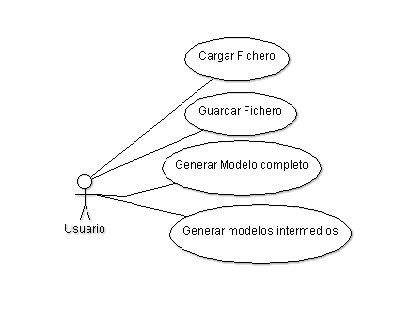
\includegraphics[width=0.9\textwidth]{imagenes/diagramas/DCU1.png}
\caption{Diagrama de casos de uso Análisis-Calibración.}
\end{figure}
\
\begin{figure}[H]
\centering
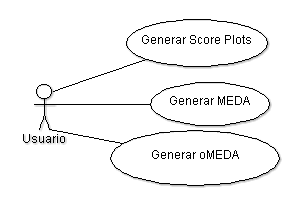
\includegraphics[width=0.9\textwidth]{imagenes/diagramas/DCU2.png}
\caption{Diagrama de casos de uso Visualización.}
\end{figure}
\newpage
\section{Diagrama de paquetes}

Este tipo de diagrama representa la estructura según las relaciones lógicas existentes así como las dependencias entre los elementos que componen el software. Cada paquete nos sirve como estructura para organizar ciertos elementos del modelo agrupándolos.
\bigskip

\begin{figure}[H]
\centering
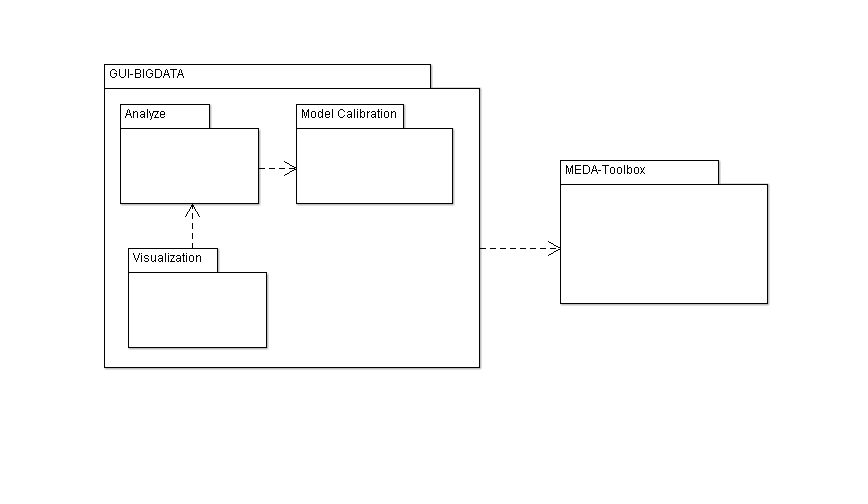
\includegraphics[width=0.9\textwidth]{imagenes/diagramas/DDP.png}
\caption{Diagrama de paquetes.}
\end{figure}

Se puede observar en el diagrama de paquetes que el paquete “Analyze” depende del “Model Calibration” lo cual quiere decir que para poder analizar los datos primero se debe calibrar el modelo mediante los parámetros de entrada. Por otra parte para poder llevar a cabo la visualización se tienen que tener los datos ya calibrados y analizados,  almacenados en una estructura de datos. Como vemos todo el conjunto de paquetes GUI-BIGDATA depende de MEDA-Toolbox que para simplificar el diagrama ha sido encapsulada en un solo paquete.
\bigskip

\section{Diagramas de actividad}

Este tipo de diagramas representan la actividad de un caso de uso, la actividad realizada por un conjunto de objetos o los flujos entre varios casos de uso.
\bigskip

Para los dos primeros casos de uso los diagramas de actividad son triviales puesto que tanto para guardar como para cargar ficheros se selecciona un fichero concreto, lo cual hace el diagrama innecesario.
\bigskip

\begin{figure}[H]
\centering
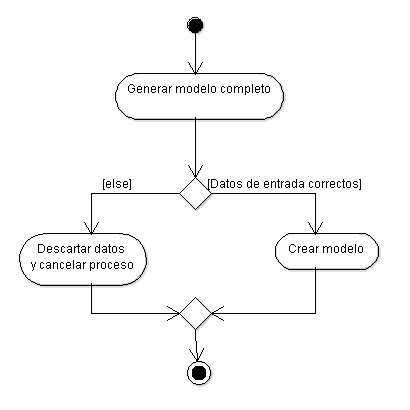
\includegraphics[width=0.9\textwidth]{imagenes/diagramas/DA1.png}
\caption{Diagrama de actividad CU-3.}
\end{figure}

\begin{figure}[H]
\centering
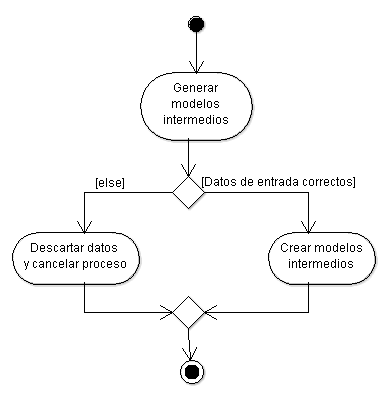
\includegraphics[width=0.9\textwidth]{imagenes/diagramas/DA2.png}
\caption{Diagrama de actividad CU-4.}
\end{figure}

\begin{figure}[H]
\centering
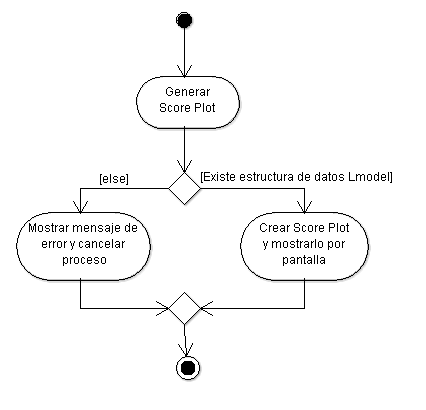
\includegraphics[width=0.9\textwidth]{imagenes/diagramas/DA3.png}
\caption{Diagrama de actividad CU-5.}
\end{figure}

\begin{figure}[H]
\centering
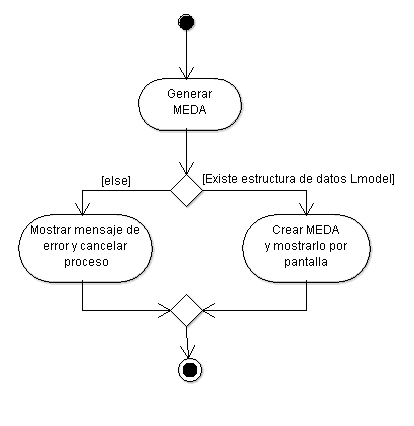
\includegraphics[width=0.9\textwidth]{imagenes/diagramas/DA4.png}
\caption{Diagrama de actividad CU-6.}
\end{figure}


\begin{figure}[H]
\centering
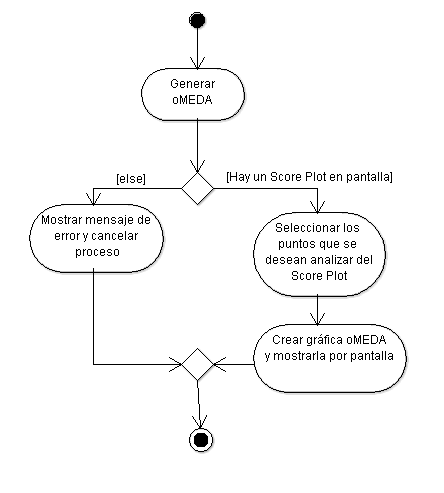
\includegraphics[width=0.9\textwidth]{imagenes/diagramas/DA5.png}
\caption{Diagrama de actividad CU-7.}
\end{figure}
